% \documentclass[reprint,superscriptaddress,prb,floatfix,showkeys]{revtex4-2}
\documentclass[10.5pt]{article}
\usepackage{lmodern}
\usepackage[utf8]{inputenc}
\usepackage{braket}
\usepackage{amsmath}
\usepackage[T1]{fontenc}
\usepackage{tgpagella}
\usepackage{graphicx}
\usepackage{caption}
\usepackage{subcaption}
\usepackage[utf8]{inputenc}
\usepackage{amssymb}
\usepackage[dvipsnames]{xcolor}
\usepackage{graphicx}
\usepackage{caption}
\usepackage{float}
\usepackage{tikz}
\usetikzlibrary{lindenmayersystems}
\usepackage[usestackEOL]{stackengine}
\newtheorem{theorem}{Theorem}[section]
\usepackage{appendix}
\usepackage[capitalise]{cleveref}
\usepackage{imakeidx}
\usetikzlibrary{calc}
\usepackage[normalem]{ulem}
\usepackage[capitalise]{cleveref}

\newcommand{\brac}[1]{\left(#1 \right)} %nice brackets
\newcommand{\bk}[1]{\langle #1 \rangle} 
\newcommand{\m}{\text{m}} %m index
\newcommand{\M}{\text{M}} %m index
\newcommand{\N}{\text{N}} %n index
\newcommand{\n}{\text{n}} %n index
\renewcommand{\a}{\textbf{\text{a}}} %a index

\linespread{1.2}

    \usepackage{geometry}
    \geometry{
     a4paper,
     left=22mm,
     right=22mm,
     top=25mm,
     bottom=30mm,
     }

\title{Learning in Memristive Neural Networks}
\date{}
\begin{document}
% \captionsetup{width=0.93\textwidth}

% \maketitle


[A change in the chosen weight of a memristor directly influences the functional form of $g_{\infty}(\boldsymbol{\Delta})$. In turn, this functional form guides the evolution toward a steady state that aligns with the desired one. It is important to note that the entire functional form is significant, not just the steady-state value of the potential drop and the corresponding conductance, as explained in Appendix A.] -> add in paper

\section*{Dynamical evolution to the steady state}
In this section, we explain more in depth the relaxation toward a steady-state of a memristor network. Specifically, we want to emphasise that in a network where the applied voltage is constant at the input nodes, the dynamical dependence on the steady-state conductance is fundamental to reach desired values of potential drops. 


For simplicity, we consider a voltage divider, as shown in \cref{fig:app_vd}, where we set $\Delta P = 0$ and $\Delta \rho = 0$. 
\begin{figure}[H]
    \centering
    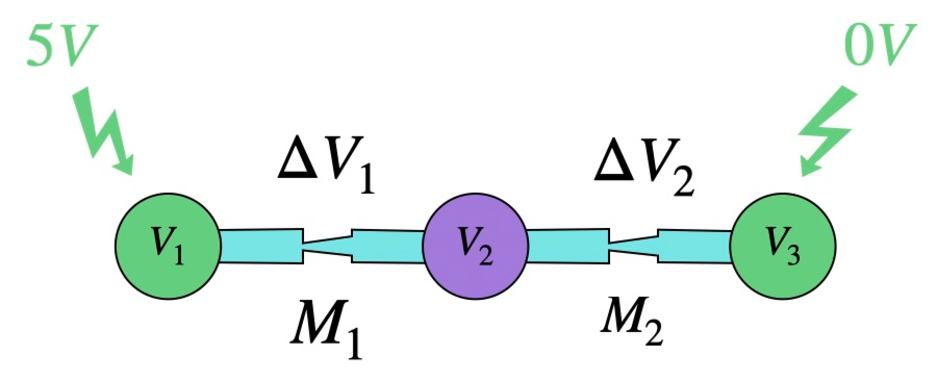
\includegraphics[width=0.5\columnwidth]{../plots/app_vd.pdf}
    \caption{}
    \label{fig:app_vd}
\end{figure} 
Therefore, the dynamical evolution of the conductance of each memristor discretized in time-steps $\Delta t$, shown in its general form in Eq. (2), reduces to
\begin{equation}
    g_{\m}\brac{t + \Delta t} = g_{\m}\brac{t} +
     \frac{g_{\m,\infty}\brac{\Delta V_{\m}(t)}-g_{\m}\brac{t}}{\tau}\Delta t,
\label{eq:conduct}
\end{equation}
with initial condition $g_{\m}(t=0)=g_0$. At each time-step, the potential drop $\Delta V_{m}(t)$ across each memristor is calculated using Kirchoff's law, that reduces to the expressions
\begin{equation}
    \Delta V_1(t) = \frac{5 g_2(t)}{g_1(t)+g_2(t)}, \ \ \ \ \ \ \ \Delta V_2(t) = \frac{5 g_1(t)}{g_1(t)+g_2(t)},
    \label{eq:potentials}
\end{equation}
found by minimizing the power dissipated by the resistances with respect to the free potential $\partial P/\partial V_2=0$.

The algorithm works as follows:

\begin{itemize}

    \item At time $t=0$, the potentials $\Delta V_1(t=0)$ and $\Delta V_2(t=0)$ are computed from \cref{eq:potentials} using the initial condition $g_1(t=0)=g_2(t=0)=g_0$.
    \item In the following time-step $t=\Delta t$, the potentials $\Delta V_1(t=0)$ and $\Delta V_2(t=0)$ are used to compute conductances $g_{\m}(\Delta t)$ using \cref{eq:conduct}.
    \item The previous step is iterated, and the system reaches the steady-state when $g_{\m}(t)=g_{\m,\infty}(t)$.

\end{itemize}

\begin{figure}[h]
    \centering
    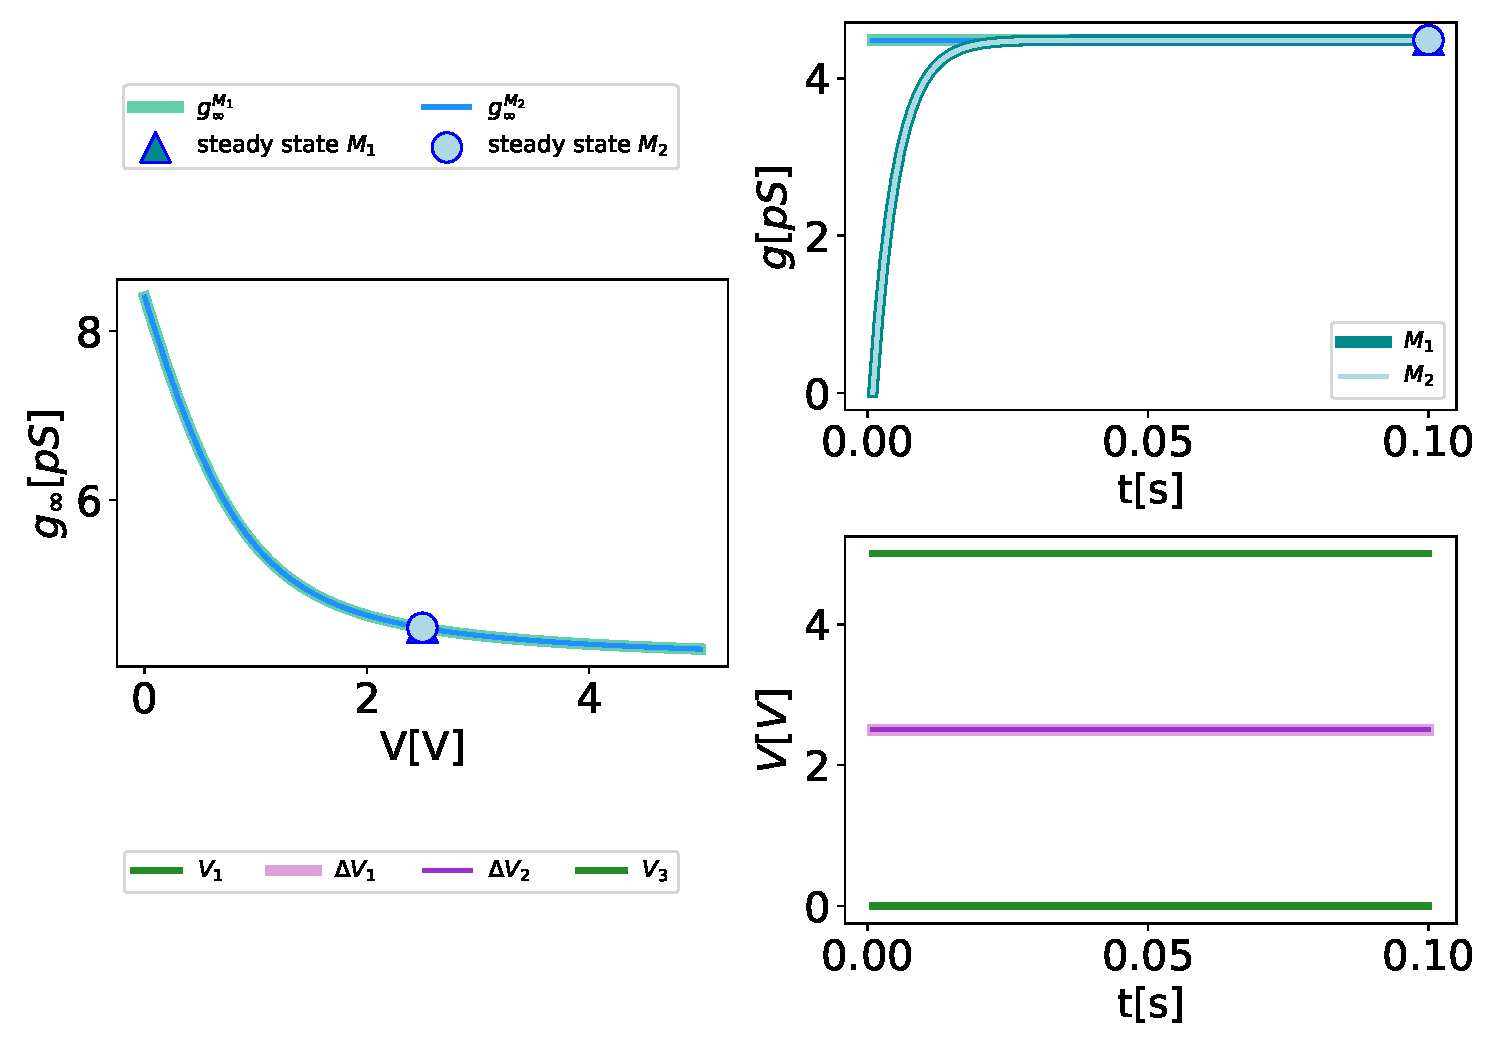
\includegraphics[width=0.8\columnwidth]{../plots/grid_initial_condition.pdf}
    \caption{Relaxation toward the steady
    state when $g_{1,\infty}(V)=g_{2,\infty}(V)$.}
    \label{fig:memristor_network}
\end{figure} 

\begin{figure}[h]
    \centering
    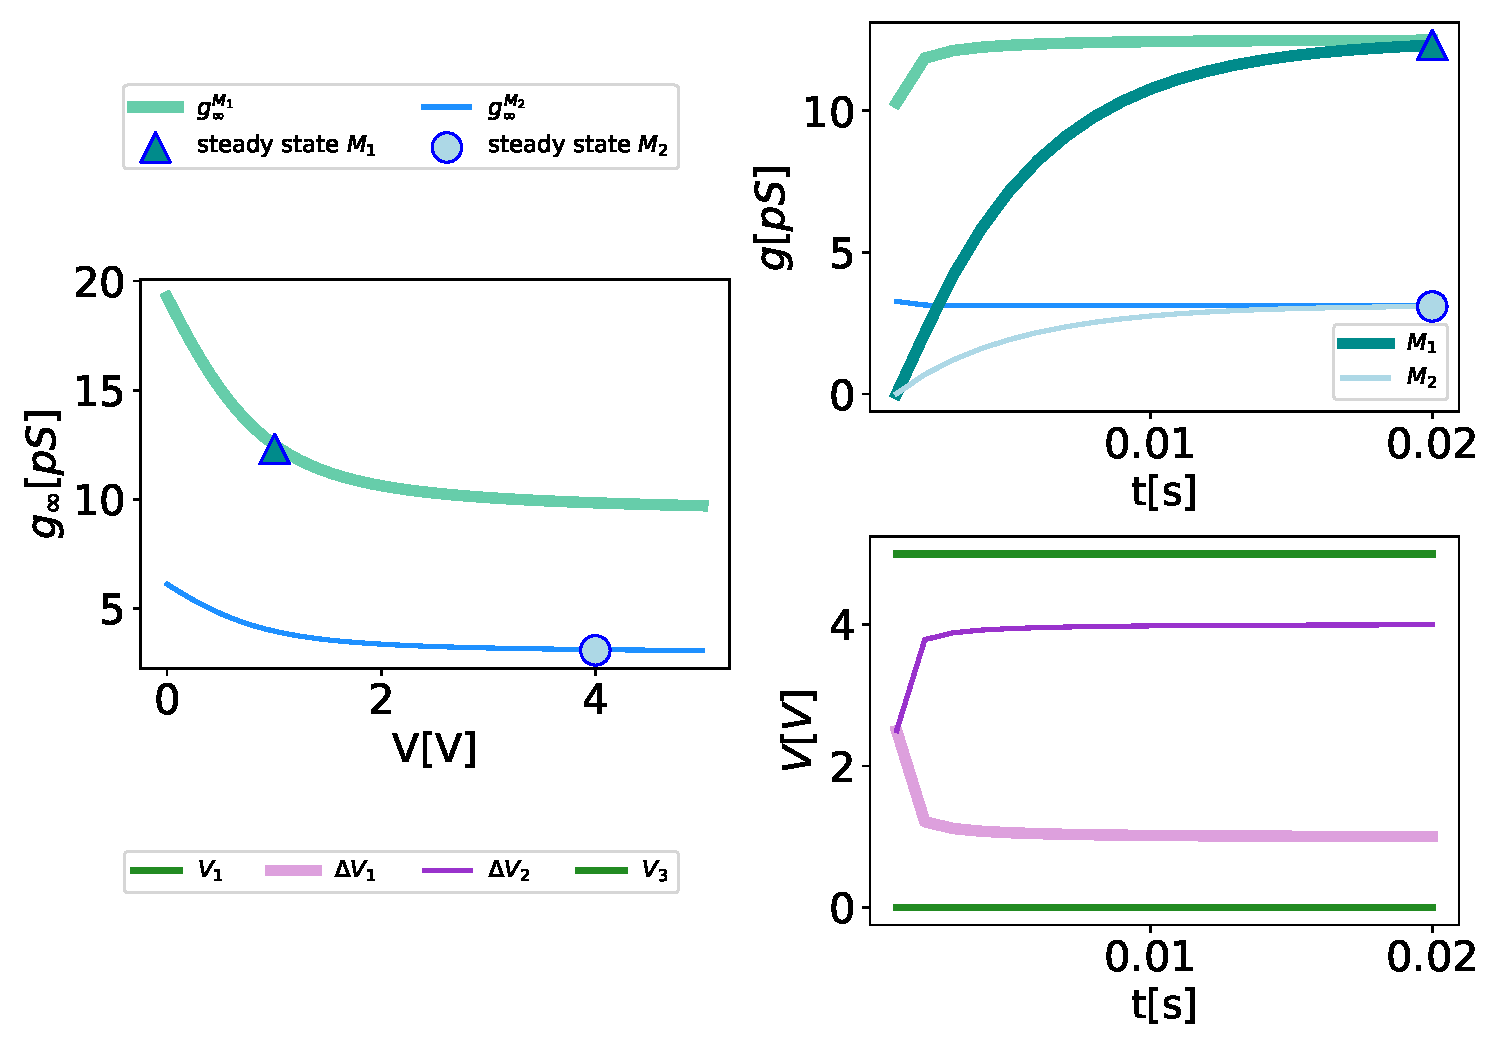
\includegraphics[width=0.8\columnwidth]{../plots/grid_trained.pdf}
    \caption{Relaxation toward the steady state when the system has been trained to give $V_2 = 4V$. The training sets the two different functional forms of $g_{\infty}$ seen in the right figure.}
    \label{fig:memristor_network}
\end{figure} 

\begin{figure}[h]
    \centering
    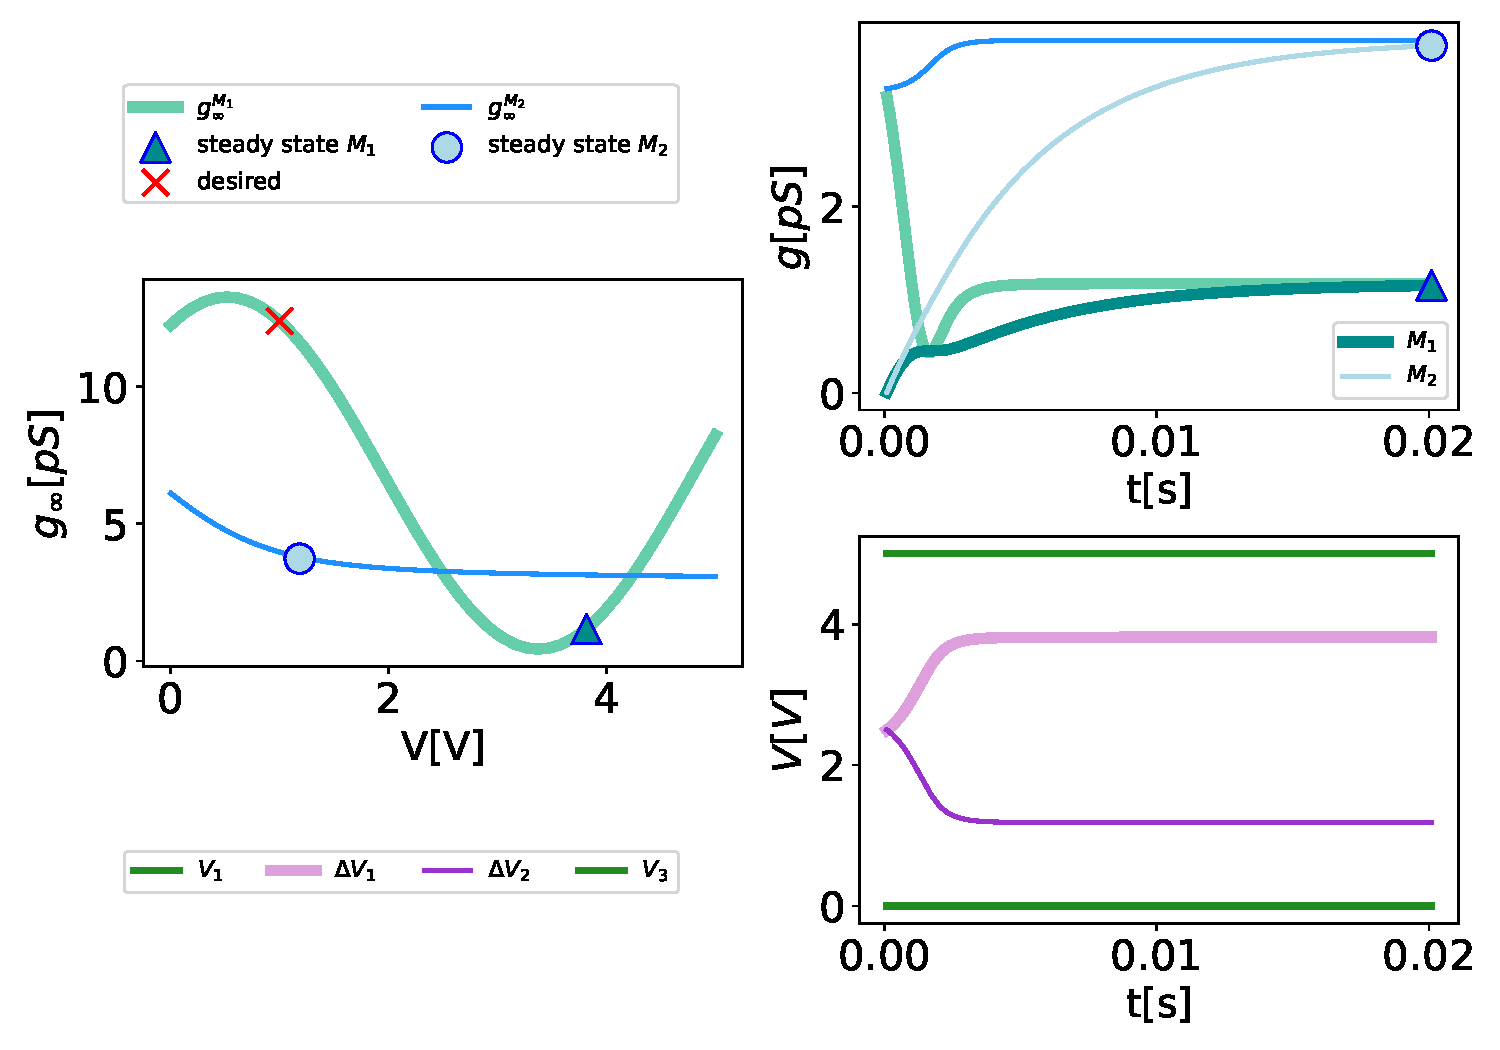
\includegraphics[width=0.8\columnwidth]{../plots/grid_trained_change_func.pdf}
    \caption{We consider the trained system in Figure 3, but we define the funtion $g_{1, \infty}$ such that it passes througth the steady state point (triangle in Figure 3), now indicated with a red cross, but with a different functional form. Due to the different functinal form, the system reaches a steady state that doesn't coincide with the desired in Figure 3.}
    \label{fig:memristor_network}
\end{figure} 

\end{document}